\chapter{An Architecture for Real-World Community Energy Control: EnergAIze}
\label{chap:energAIze}
\label{chap:lifecycle}
\markboth{An Architecture for Real-World Community Energy Control}{An Architecture for Real-World Community Energy Control}
\newlength{\architectureoriginalparskip}
\setlength{\architectureoriginalparskip}{\parskip}
\setlength{\parskip}{0pt}
\newlength{\architectureoriginaltextfloatsep}
\newlength{\architectureoriginalintextsep}
\newlength{\architectureoriginalcaptionskip}
\setlength{\architectureoriginaltextfloatsep}{\textfloatsep}
\setlength{\architectureoriginalintextsep}{\intextsep}
\setlength{\architectureoriginalcaptionskip}{\abovecaptionskip}
\setlength{\textfloatsep}{12pt plus 2pt minus 2pt}
\setlength{\intextsep}{12pt plus 2pt minus 2pt}
\setlength{\abovecaptionskip}{6pt}
\raggedbottom
\edef\architectureoriginalclubpenalty{\the\clubpenalty}
\edef\architectureoriginalwidowpenalty{\the\widowpenalty}
\clubpenalty=10000
\widowpenalty=10000

The preceding chapter reviewed approaches to \gls{rec} energy control and identified gaps in their use in real-world installations. This chapter presents the architecture of EnergAIze, connecting control in buildings and \glspl{rec} to controller development, experiment orchestration, and deployment.

\section{Energy Control in Buildings and Communities}
\label{sec:energAIze-overview}
\label{sec:energaize-overview}
\label{sec:energAIze-functional-view}
\label{sec:energaize-community-view}

Households need their vehicles ready for travel, their rooms at a comfortable temperature, and their appliances to complete their work. Meeting these needs leaves choices about when electricity is consumed or stored, especially where a building also produces some of its own energy. To make those choices, a controller needs information about the services people require, the resources available to deliver them, and the limits within which they can operate. EnergAIze connects this information to the equipment through which a decision takes effect.

Consider the vehicle introduced in Chapter~\ref{chap:introduction}, arriving home at 18:00 with a \gls{soc} of 30\% and a target of 80\% by 08:00. The charger reports that the vehicle is connected, vehicle information supplies its \gls{soc}, and the household meter shows how much power the other loads are using. Together with the departure requirement and the available charging capacity, these observations allow the controller to choose a charging power. That decision is sent through the installation's control interface, and subsequent measurements report the power delivered and the progress towards the target.

\Cref{fig:energaize-building-loop} presents this flow. In the figure, \emph{State of the Environment} denotes the observations assembled for a decision. EnergAIze uses them to determine actions for the connected resources. Measurements and actions pass through the local control system or external service provider associated with the equipment.

\begin{figure}[htbp]
\centering
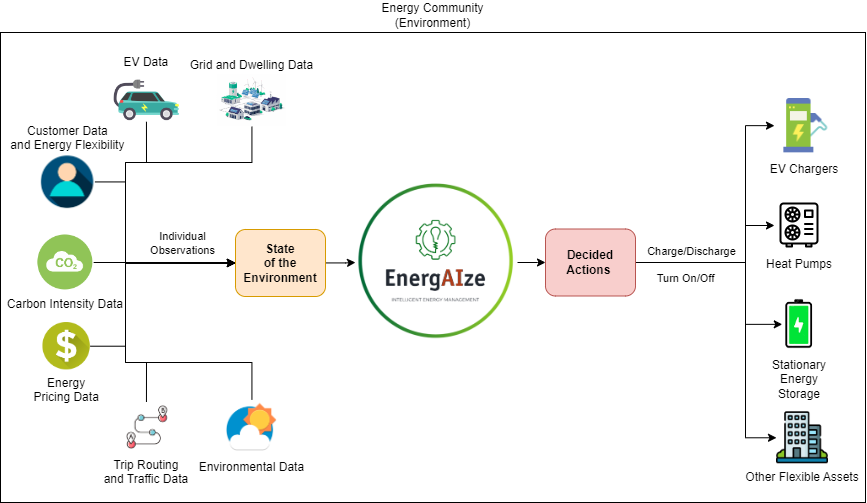
\includegraphics[width=\linewidth]{energaize-information-actions.png}
\caption[Information and actions in EnergAIze.]{Information and action flow. Source: author's master's dissertation.}
\label{fig:energaize-building-loop}
\end{figure}

The inputs shown in \cref{fig:energaize-building-loop} fall into seven categories, according to the information they contribute to a decision:

\begin{description}[font=\normalfont\bfseries,leftmargin=0pt,itemsep=0.25\baselineskip,topsep=0.4\baselineskip]
\item[User requirements and flexibility.] Requested services and the freedom to adjust their delivery, such as a vehicle's departure time and target \gls{soc}, a comfort range, or an appliance's operating window.
\item[Vehicle data.] Battery \gls{soc}, charging status, and battery capacity. These describe the vehicle's current condition and help determine the energy needed for its next use.
\item[Building and grid data.] Demand, \gls{pv} production, storage state, grid exchange, and connection limits. These describe the installation's energy balance and the capacity available for flexible resources.
\item[Electricity prices.] Purchase prices and, where applicable, export remuneration or \gls{rec} exchange prices. Their variation over time informs the cost of a charging or storage decision.
\item[Carbon intensity.] Emissions associated with electricity supply. This information allows the controller to consider the emissions consequences of using grid electricity at different times.
\item[Environmental data.] Weather conditions and forecasts, including temperature and solar irradiance. These help anticipate changes in renewable production and weather-dependent demand.
\item[Travel and traffic data.] Planned journeys, routes, and traffic conditions. These can inform estimates of vehicle arrival, departure, and energy use, complementing the requirements supplied by the user.
\end{description}

These categories can contain measurements, user declarations, configuration values, or forecasts. The vehicle's current \gls{soc} is a measurement; its required departure charge is a user requirement; its expected return time may be a forecast. Keeping these roles distinct allows the controller to use each value appropriately. The input selection for each experiment is retained in the configuration records described in Appendix~\ref{app:controller-configurations}.

The loop repeats as conditions change. Cooking and heating can reduce the power available for charging; when those loads subside, charging can increase. At each decision interval, the controller receives updated measurements and accounts for the time remaining before departure. The measurements also show how closely the delivered power followed the request.

Across a \gls{rec}, this arrangement is repeated for buildings with different equipment and daily routines. One household may have \gls{pv} panels and a battery, another a vehicle charger, and a workplace several charging points. Each building has a controller and associated data processing, configured for its resources. Measurements and actions remain linked to that building, while information relevant to the \gls{rec} can be shared among the participating controllers.

\Cref{fig:energaize-community} extends the first view to several buildings. Each local controller receives observations from its building and returns actions to its equipment. In the illustrated deployment, a \gls{rec} server supplies shared information, including time, weather, carbon intensity, and electricity prices. The actor network represents the learned controller executed for each building. This organisation also accommodates the hierarchical methods developed in Chapter~\ref{chap:control-benchmark}, where a \gls{rec} controller supplies guidance for local decisions.

\begin{figure}[htbp]
\centering
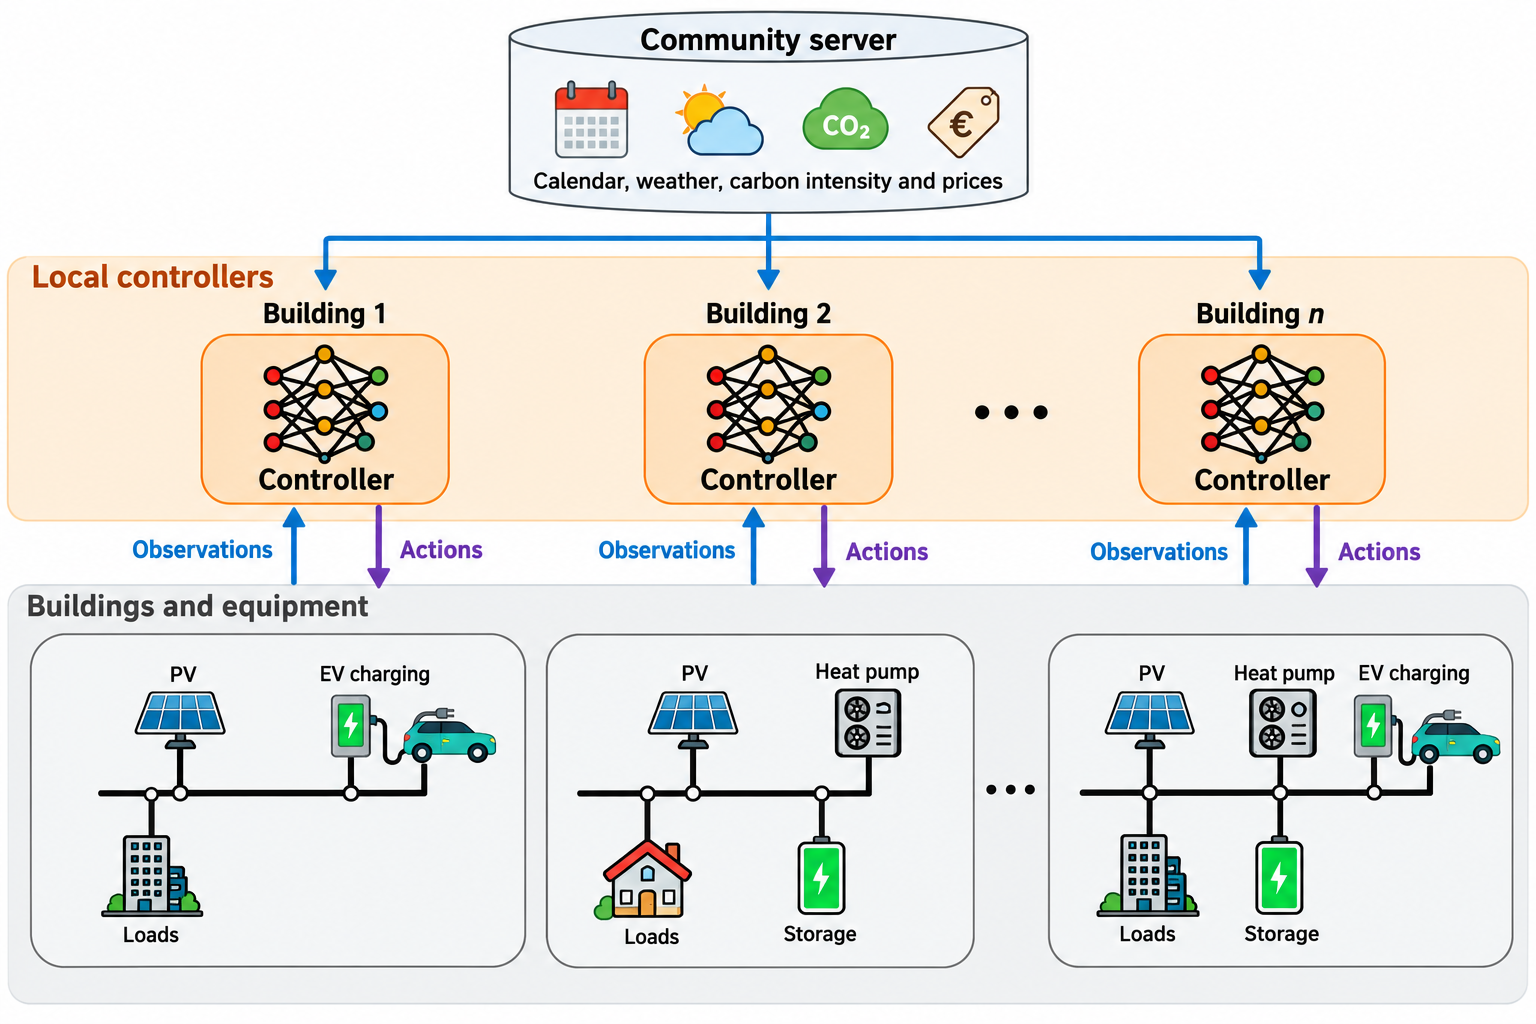
\includegraphics[width=\linewidth]{energaize-community-deployment-revised.png}
\caption[Building controllers within a \gls{rec}.]{\gls{rec} deployment. Adapted from the author's master's dissertation.}
\label{fig:energaize-community}
\end{figure}

\Needspace{3\baselineskip}
The blue arrows carry observations from each building and the shared services into its controller; the purple arrows carry the resulting actions to its equipment. For the charging example, local information establishes what the household can do, while \gls{rec} information helps determine when that flexibility is useful. On a different day, when the vehicle remains connected until late afternoon, the controller can account for renewable production available elsewhere in the \gls{rec}. When many vehicles arrive together, spreading charging over their connection windows can limit the combined demand.

Organising data processing and control around each building gives installation-specific work a clear scope. Connecting a new charger changes that building's configuration and available actions. Adding a building introduces another local loop and updates the \gls{rec} information used for coordination. Processing close to the data source can reduce communication and keep detailed measurements within the local processing path. The controllers in \cref{fig:energaize-community} coexist with shared services and provider platforms, with placement determined by each installation.

\begin{samepage}
Putting these local control loops into operation involves two complementary paths. During \emph{runtime}, incoming observations support a decision whose consequences are measured at the installation. During \emph{development}, data and simulation provide the conditions in which a controller is prepared and evaluated for that role. The runtime path is considered first, establishing what the controller must receive and produce. The development path then explains how such a controller is obtained, followed by the infrastructure that runs the experiments and loads the selected model into service.

\end{samepage}

% Keep the runtime overview in the chapter's portrait page orientation.
\section{Runtime Architecture}
\label{sec:energaize-runtime}

The information and action flow described above requires several services to work within each decision interval. Measurements must reach the controller in a usable form, the controller must choose an action, and that action must reach the equipment with the applicable checks. The \gls{cw} cloud platform and other \gls{iot} interfaces connect the equipment to these services through \glspl{api}. \Cref{fig:energaize-overview} shows how EnergAIze assigns these responsibilities, expanding one building to expose its runtime components.

\begin{figure}[H]
\centering
\makebox[\linewidth][c]{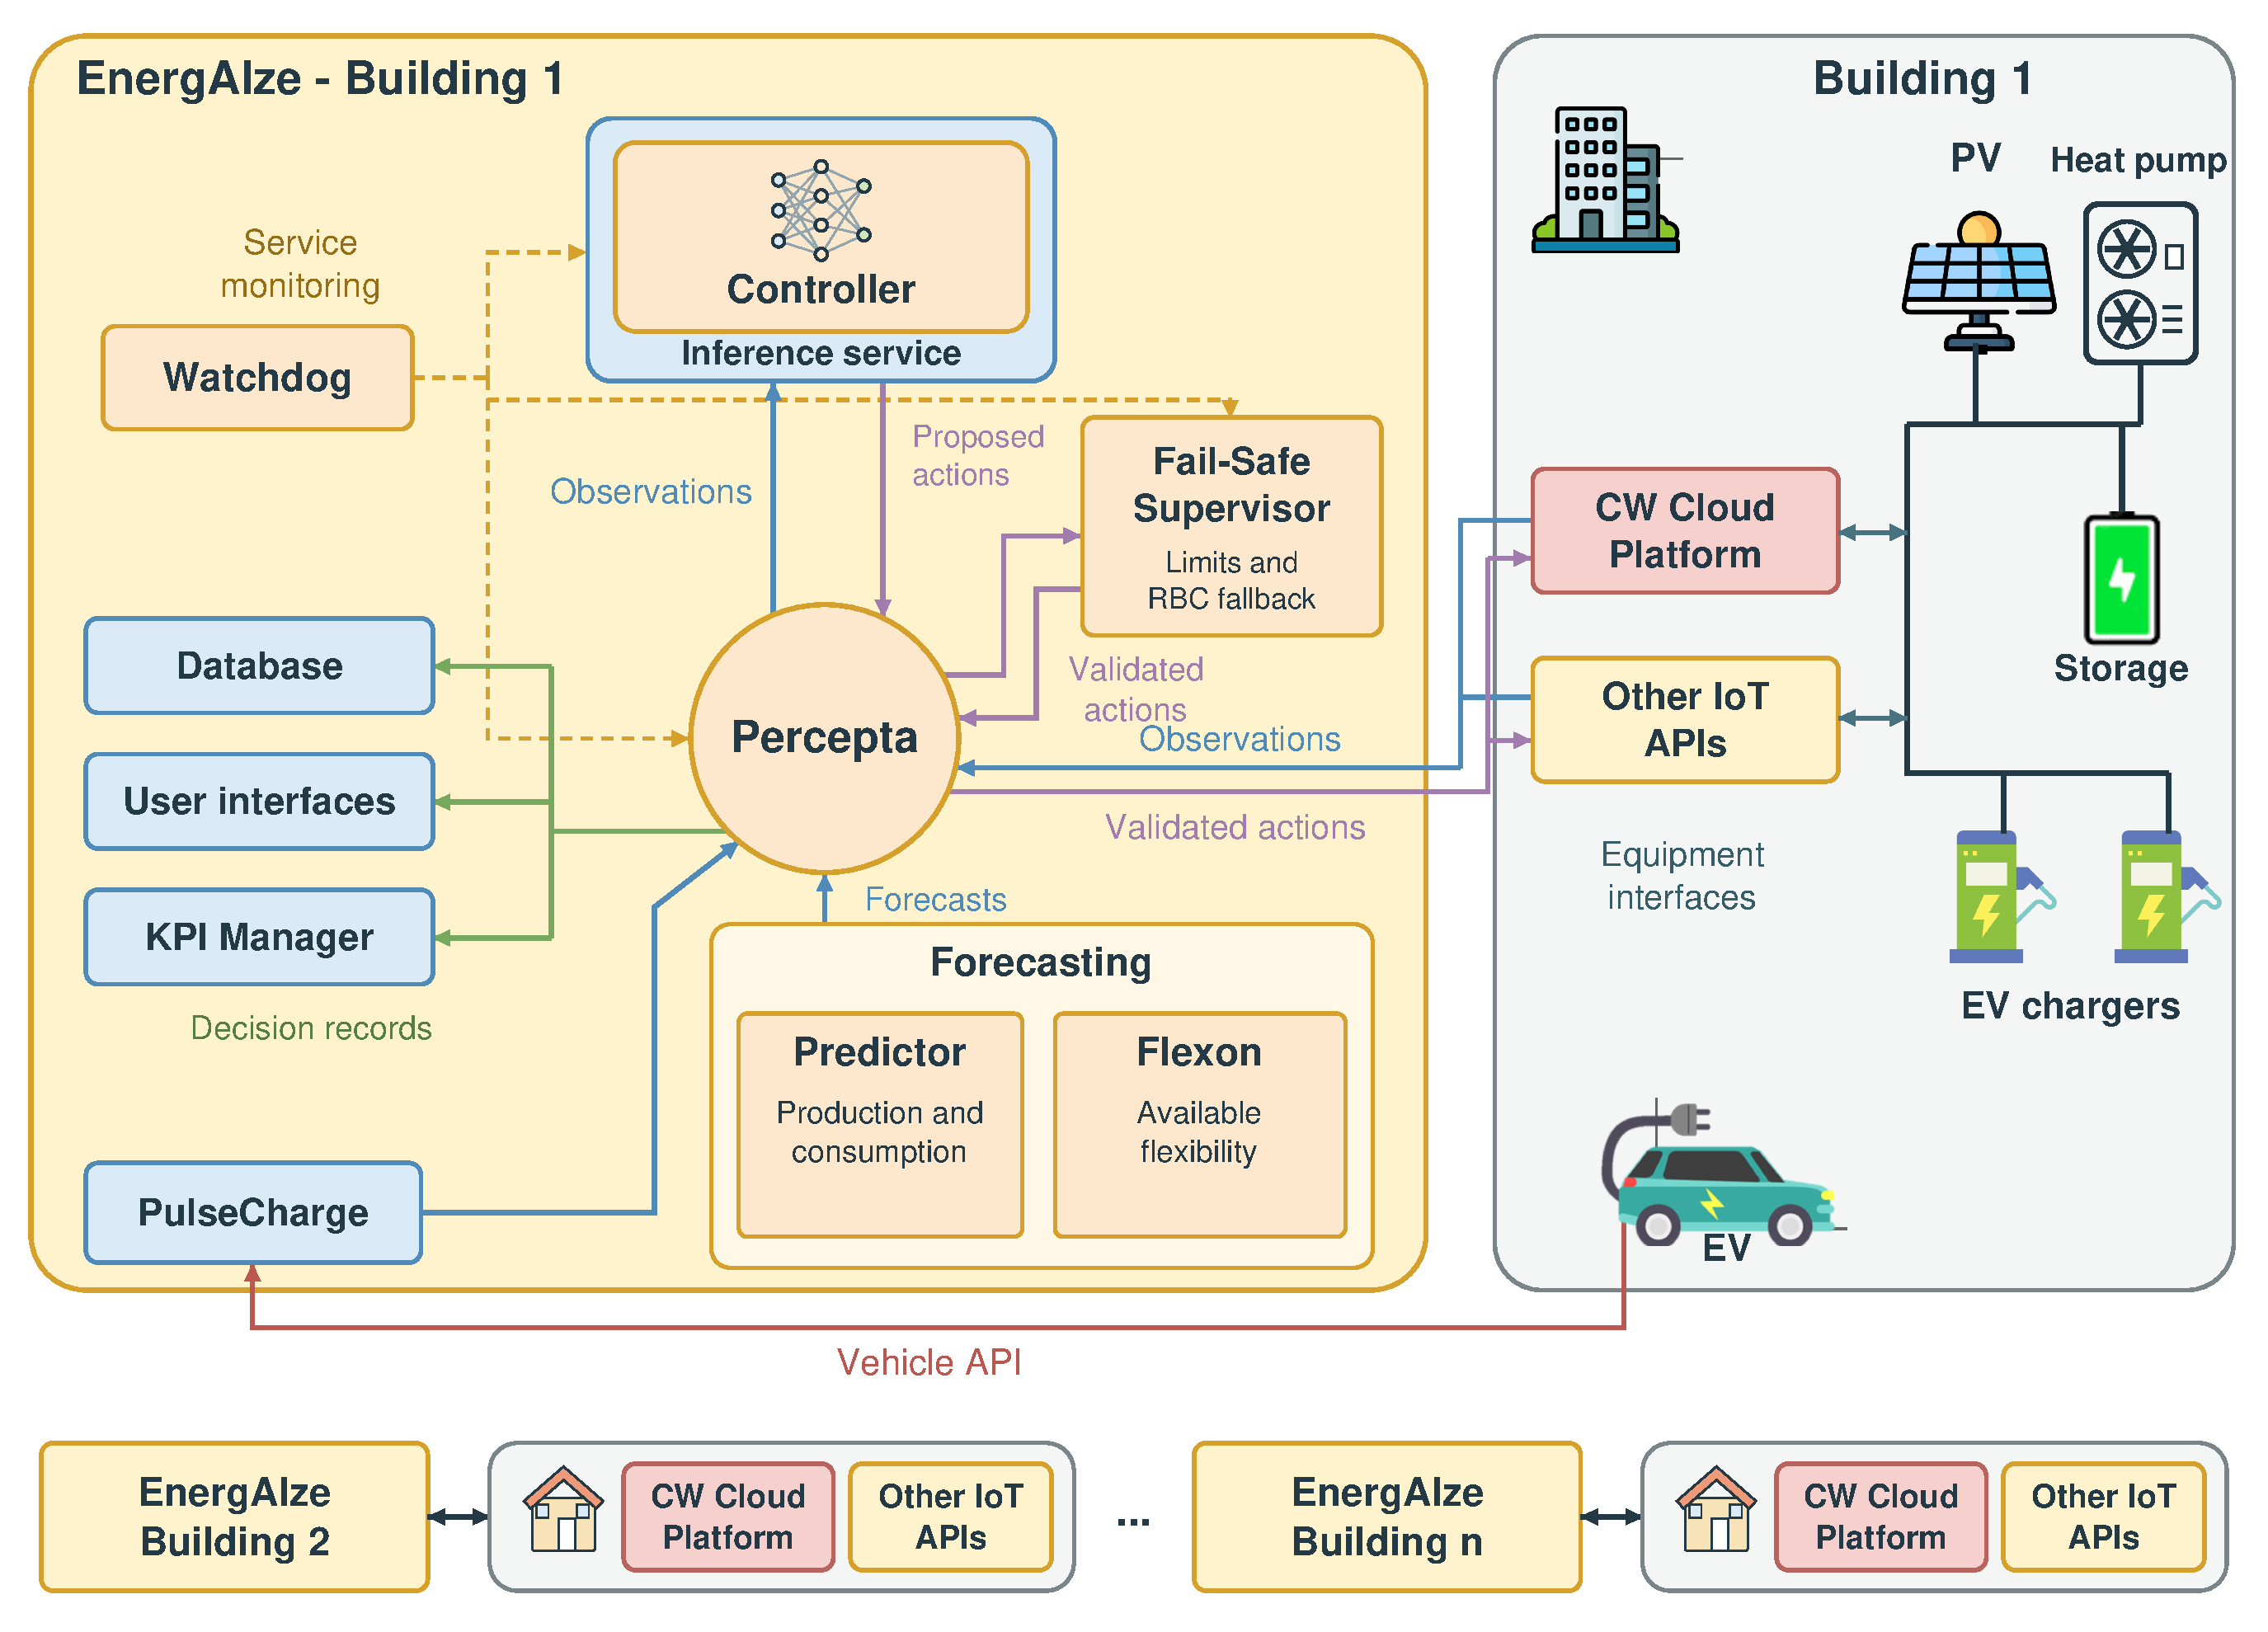
\includegraphics[width=1.1\linewidth]{energaize-runtime-revised.pdf}}
\caption[Runtime architecture of EnergAIze.]{Runtime architecture of EnergAIze, expanded for one building.}
\label{fig:energaize-overview}
\end{figure}

\begin{samepage}
On the right of the figure, the \gls{cw} cloud platform and other \gls{iot} interfaces connect the physical equipment to EnergAIze. On the left, Percepta processes incoming observations and routes outgoing actions. Vehicle information and forecasts support the controller, while action validation, service monitoring, and operational records accompany its decisions. This organisation underlies the integrations described in the EnergAIze publications and \gls{opeva} demonstrator \parencite{fonseca2024energAIze,fonseca2025realworldrec,opeva2026d63}.

\end{samepage}

\begin{samepage}
Installation configuration links these components to equipment, measurement sources, commands, and operating limits. A model contract specifies the controller's inputs and outputs; Section~\ref{sec:energaize-contract} describes its passage into runtime. The architecture and the roles of its components were conceived and designed by the author, who also guided the collaborative research and student projects through which several components were implemented. Their implementation contributions are acknowledged in the associated publications and the Statement on Co-Authored Work.

\end{samepage}

\subsection{The Controller and Its Inference Service}
\label{sec:energaize-algorithms}

At the centre of the runtime is the controller, shown within the inference service in \cref{fig:energaize-overview}. It determines how the resources under its control should operate during the next interval. The surrounding services supply information, apply its decisions, and report their consequences. The control methods investigated in Chapters~\ref{chap:control-benchmark} and~\ref{chap:ti-marl} occupy this position in the architecture.

For the household vehicle, the immediate choice is the charging power to request. Its consequences extend beyond the next interval: charging now contributes towards the departure requirement but also increases household demand, while delaying charging preserves capacity now and leaves less time to deliver the remaining energy. A stationary battery introduces a related choice. Discharging it may support the household during a busy period, although the energy then used will no longer be available later. The controller considers these resources together, using the observations and forecasts selected for its decision problem.

The control methods reviewed in Chapter~\ref{chap:related-work} can occupy this role through a common observation and action interface. A \gls{rbc} applies its configured rules, an optimisation method solves the current scheduling problem, and a learned controller evaluates its policy. The reinforcement-learning methods studied in this thesis use that interface during both development and operation, keeping decisions associated with the same resources and service requirements.

At \gls{rec} level, the decisions made in one building influence the conditions experienced by others. Several households postponing charging until the same low-price interval can create a new peak. Coordination requires the controller formulation to represent the relevant \gls{rec} information and relationships, whether through shared observations, the learning process, or guidance from a \gls{rec} controller. The runtime provides the communication and resource associations needed by the selected method. The progression from building decisions to coordinated and hierarchical control is developed in Chapter~\ref{chap:control-benchmark}; Chapter~\ref{chap:ti-marl} examines how the controller can accommodate changes in the participating resources.

The inference service executes the model selected for this role. It receives the prepared observations, applies the input processing declared by the model contract, evaluates the model, and returns named actions. The algorithm determines the decision; the service supplies the software interface through which that decision becomes available to the rest of EnergAIze. A compatible rule-based policy can occupy the same interface. Keeping the observation and action interpretation with the model allows a selected controller to be loaded without reconstructing its processing by hand.

The returned actions are proposals for the current interval. Before they reach the charger or battery, they pass through the validation and provider interfaces described below. Subsequent measurements close the loop by revealing what the equipment actually did. Preparing the inputs for this sequence begins with the data-integration service.

\subsection{Data Integration and Routing: Percepta}
\label{sec:energaize-percepta}

The measurements required for a decision can arrive through different interfaces and at different times. A building energy-management platform may expose meter readings and battery status, a charging platform may report connection and charging power, and a vehicle service may provide \gls{soc}. The stream-processing component, Percepta, handles the integration and processing of these sources so that the controller receives observations associated with the correct building and resources \parencite{percepta2025}.

Source-specific receivers obtain the incoming data, and translators map their fields into the representation used by the installation. Subsequent processing aligns the values used for a decision interval. For example, charging power reported in watts and household demand reported in kilowatts must be expressed consistently before they enter a common calculation. Their timestamps also matter: a charging measurement taken before the vehicle disconnected describes a different condition from the latest connection status. The data-processing path retains these associations when assembling the controller's observations.

In the \gls{opeva} integration, the Data Provider implements this path through receivers, translators, queues, an accumulator, and a manager that prepares the inference request \parencite{opeva2026d63}. The same integration work supports the retrieval of historical records for development. On the action path, a forwarder converts the validated action into the format and destination required by the equipment provider. This arrangement places provider-specific communication at the boundary of the system, allowing the controller to work with the observation and action names defined for the installation.

\subsection{Vehicle Information: PulseCharge}
\label{sec:energaize-pulsecharge}

Vehicle information extends what can be learned from the charger. The vehicle-data service, PulseCharge, retrieves information such as \gls{soc} and charging status through manufacturer interfaces, subject to the information available for the connected vehicle. It handles the corresponding authentication and periodic data retrieval, then makes that information available to the data-processing path.

In the running example, the charger establishes that a vehicle is connected, while PulseCharge can supply the 30\% \gls{soc} needed to determine how much energy remains to be delivered. These sources describe the same charging session from different points: one reports the charger and its power, the other the vehicle and its battery. Associating them with the correct vehicle and charger allows the controller to interpret them together. The charging platform remains the interface through which the charging action is applied.

\subsection{Production and Consumption Forecasting}
\label{sec:energaize-prediction}

The production and consumption forecasting services, represented by \emph{Predictor} within the forecasting group in \cref{fig:energaize-overview}, supply expected conditions over the period considered by the controller. Production forecasts estimate \gls{pv} output; consumption forecasts estimate the demand against which charging or battery operation will take place. Their inputs can include historical measurements, weather information, and calendar variables. Percepta makes the resulting forecasts available alongside the latest observations, with the forecast horizon and time interval identifying the period they describe.

For the vehicle arriving at 18:00, a forecast of high household demand can support spreading charging over the night. If the vehicle remains at home on another day, a forecast of substantial midday production may favour charging during that period. Each forecast concerns a future quantity whose realised value will later be measured. As new observations arrive, subsequent decisions can account for the difference between the expected and actual conditions. This connection keeps forecasts within the ordinary sequence of measurement, decision, and response.

\subsection{Flexibility Forecasting: Flexon}
\label{sec:energaize-flexon}

The flexibility-forecasting component, Flexon, estimates the flexibility expected to be available from participating resources. Within the forecasting role shown in the runtime figure, it supplies information about opportunities to adjust consumption or storage. For vehicle charging, this includes anticipating when a vehicle will be available and the energy associated with its expected use. The controller can then consider whether the anticipated connection window offers room to move charging towards a more favourable period.

User requirements establish the service to be delivered during the current connection. In the example, the driver requests 80\% by 08:00. If an earlier departure is specified, the available charging window becomes shorter even when previous journeys suggest a later departure. The controller receives both the forecast used to anticipate availability and the current requirement that its decisions must satisfy. Production and consumption forecasts describe the energy conditions around this opportunity; Flexon describes the flexibility expected to be available within it.

\subsection{Action Validation: Fail-Safe Supervisor}
\label{sec:energaize-supervision}

The Fail-Safe Supervisor is a separate component between the controller's proposed action and the request sent to the equipment. It checks the proposal against the installation's operating limits and current resource information, including charger ratings, battery limits, and available connection capacity. A proposal within those limits passes through unchanged; where a request exceeds the available capacity, the supervisor limits it before forwarding. In the \gls{opeva} middleware, validation precedes the forwarder that constructs the provider request \parencite{opeva2026d63}.

Each part of this path has a distinct responsibility. The controller's feasibility mechanisms account for the constraints represented by its method, while the inference service applies the output bounds and resolution declared for the model. The supervisor checks the resulting request against the operating conditions reported by the installation. Provider platforms and equipment retain their own protections when executing the validated action. This separation preserves the distinction between policy proposals, supervisory intervention, and equipment response developed in Section~\ref{sec:ch2-safety-literature}.

For the household vehicle, an increase in other loads may leave less power available than the controller requested. The supervisor reduces the charging command to the available capacity, and the next measurements show how much energy was delivered. Subsequent decisions then account for the energy still required before 08:00. The record of the original proposal and its correction makes it possible to examine both the immediate limit and the effect on departure readiness.

If the algorithm stops or produces no inference output for the current interval, the supervisor uses a lightweight \gls{rbc} to provide a fallback action. Its configured rules use the available operating information and remain subject to the installation's limits. The supervisor logs these fallback decisions as well as adjustments to policy proposals. The resulting records show when the learned controller supplied the action, when supervision changed it, and when control continued through the fallback.

\subsection{Service Monitoring: Watchdog}
\label{sec:energaize-watchdog}

The Watchdog monitors the services involved in the control loop, including data processing, controller execution, and supervision. It identifies interruptions so that the affected service can be examined and restored. The supervisor provides the immediate fallback when an inference output is unavailable; the Watchdog makes the service interruption visible to the operator. Its scope follows the dependencies: losing one vehicle-data source affects that vehicle's observations, while losing a shared inference service may affect several buildings. Resuming learned control requires the relevant observations and inference outputs to be available again.

Data availability also matters while the services themselves remain running. In the documented \gls{opeva} middleware, an absent measurement can be completed with the previous value when preparing an interval \parencite{opeva2026d63}. Its source time remains important when deciding how that value can be used. A delayed price update and an unavailable battery \gls{soc} have different implications for the charging decision. The response depends on the information needed for the requested action and the alternative control behaviour configured for the installation.

\subsection{Operational Records, User Interfaces, and KPI Manager}
\label{sec:energaize-records}

The database retains observations and decision records so that the course of operation can be examined. These records associate the controller version and its observations with the proposed action, any supervisory adjustment or fallback, the validated action, the provider response, and subsequent measurements. For the vehicle, they allow a reduction in charging power to be traced to the policy, the supervisor, or the equipment. Keeping that distinction through the session connects each intervention to the energy delivered before departure.

The graphical user interfaces give operators access to the current state of the installation and its operational records. They provide a way to inspect the participating resources, follow their measurements and actions, and examine interruptions reported through monitoring. An operator investigating unexpectedly slow charging can therefore relate the requested power to the vehicle state and the limits applied along the control path.

The \gls{kpi} Manager calculates \glspl{kpi} from the recorded operation. Electricity cost and peak demand can be examined at building and \gls{rec} level, alongside the vehicle's \gls{soc} at departure. The intervention records show when those outcomes were obtained with corrections or fallback control. The same operational records supply data and cases for subsequent training and evaluation.

\section{Controller Development}
\label{sec:energaize-development-runtime}
\label{sec:lifecycle-architecture}

The runtime architecture establishes what a controller receives, how its proposals reach the equipment, and how their consequences are recorded. Development prepares the controller for that role. Historical data and installation configuration provide the starting point, while simulation allows candidate policies to encounter successive conditions and be evaluated against the services they should deliver. The same process supports later retraining when operational records reveal conditions that call for a revised controller.

\Cref{fig:energaize-development} follows this controller through development. Installation records~(1) and \gls{rec} configuration~(2) define the scenarios~(3). Training~(4) and evaluation~(5) lead to the selected model bundle~(6), which reappears at the start of the deployment view in \cref{fig:energaize-deployment}. The computing infrastructure in Section~\ref{sec:orchestration} executes the training and evaluation stages as experiments.

\begin{figure}[htbp]
\centering
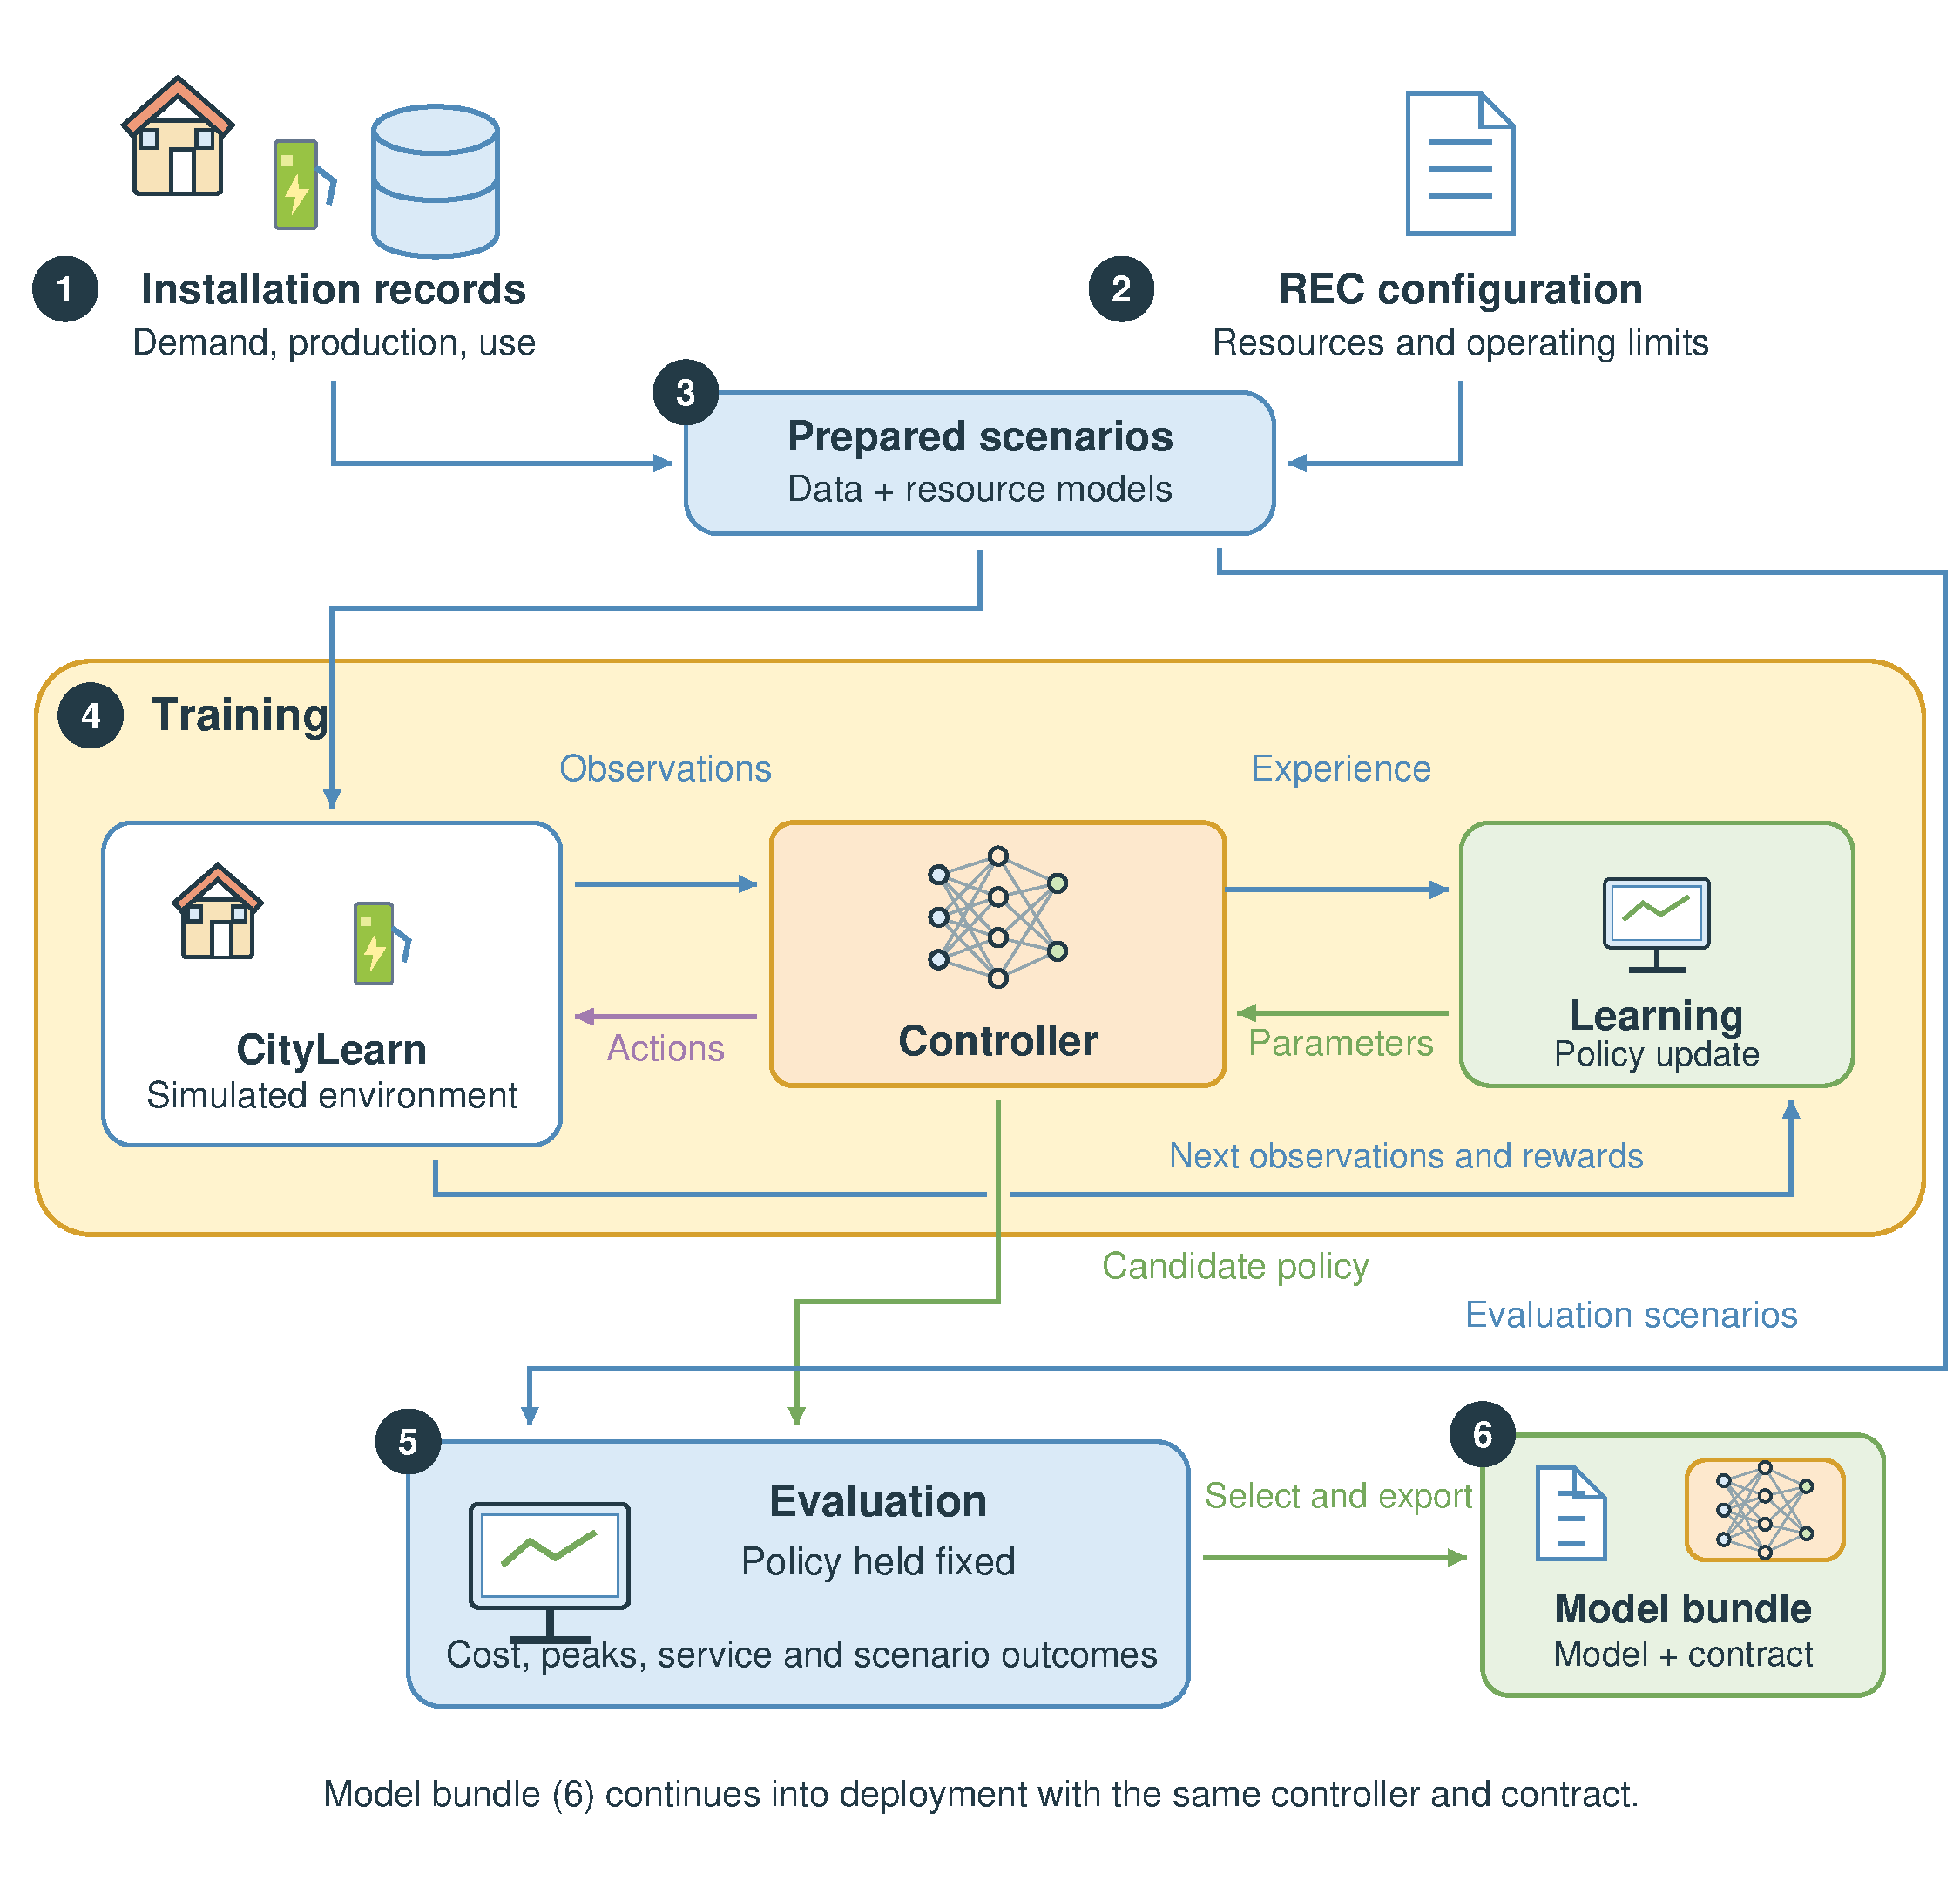
\includegraphics[width=\linewidth]{energaize-controller-development.pdf}
\caption[Controller development through simulation and evaluation.]{Controller development, with the model bundle~(6) continuing into the deployment view.}
\label{fig:energaize-development}
\end{figure}

\subsection{Data Preparation and Simulation Scenarios}
\label{sec:energaize-scenarios}

The household meter, vehicle service, and charger introduced in the runtime view also provide records from which development scenarios can be constructed. These records describe when energy was consumed, when a vehicle was present, and how its charging progressed. Data preparation aligns timestamps, units, and sampling intervals, identifies missing periods, and separates the records used for training from those reserved for evaluation. The \gls{rec} configuration identifies its buildings, equipment, capacities, and operating limits. These describe the setting in which the selected control method is developed.

The building-energy simulator, CityLearn, uses these inputs to represent the environment in which controllers act \parencite{nweye2025citylearnv2}. Vehicle and charger modelling was extended through EVLearn \parencite{fonseca2025evlearn}, and the CityLearn v3 development presented in Chapter~\ref{chap:simulator} supplies the experimental environment used throughout this thesis. Historical demand and production describe the conditions around a decision, while resource models calculate how the controllable equipment responds to it.

The distinction matters for the charging example. Recorded household demand can supply the background load for the evening, but the vehicle's \gls{soc} must evolve according to the actions chosen by the controller being tested. Replaying the recorded charging trajectory would prevent a different decision from changing the outcome. The vehicle model instead updates the stored energy as charging proceeds, subject to its parameters and the charger limits. The next observation reflects that response, allowing the controller to reconsider its decision as the departure approaches.

Supervisor records identify intervals in which a proposal was limited or a fallback supplied the action. These intervals help select conditions to reproduce during development, such as a recurring evening capacity shortage or an interruption in inference. When operational records are used directly as learning experience, the proposed action, validated action, and measured response remain associated. This retains the quantities needed to account for intervention in the learning method, following the distinction in Section~\ref{sec:ch2-constrained-foundations}.

A scenario fixes the conditions of this interaction. It identifies the buildings and resources, the available observations and actions, the external data, and the events encountered during the episode. The arrival at 18:00 and requirement of 80\% by 08:00 can be held constant while several controllers are compared. An earlier departure, a lower connection limit, or an additional vehicle creates a further scenario. These variations let the development process examine particular changes while preserving the settings needed to interpret their consequences.

The scenario also defines the correspondence with runtime. An observation of \gls{soc} belongs to a specified vehicle, and a charging action belongs to a specified charger with a defined unit and range. Forecasts describe information available when the decision is made. Maintaining these associations during simulation prepares the controller for the data and action interfaces through which it will later operate.

\subsection{Controller Training and Evaluation}
\label{sec:energaize-training-evaluation}

With the environment established, \gls{rl} proceeds through repeated interaction. The controller receives the current observations and selects actions for the represented resources. The simulator applies those actions, advances the resource states, and returns the next observations and a reward. The learning procedure uses this experience to adjust the policy. Over successive episodes, the controller encounters the consequences of its choices across complete operating periods.

In the household example, selecting a low charging power may reduce demand during a busy interval, yet leave more energy to be supplied later. The simulated trajectory exposes both effects. The reward expresses the objectives used during learning, while the environment and the controller's feasibility mechanisms represent the applicable constraints. Costs, peaks, and service outcomes can then be examined over the resulting charging session. Their precise formulation depends on the method studied and is developed in the control chapters.

Multi-agent training extends this interaction to the \gls{rec}. Each agent acts for the resources assigned to it, and the environment calculates the combined effect of those actions on buildings and shared quantities. The learning procedure may use information from several agents, even where the resulting controller uses local observations during execution. The development configuration records that distinction: information available to training and information required by the deployed policy have different roles. The runtime interface is determined by the latter.

Evaluation applies a candidate policy with its parameters fixed under scenarios kept separate from training. Common scenarios and information allow comparison with rule-based and other control methods. Energy and service outcomes are read alongside supervisory corrections and fallback use, with the same protection settings retained across a comparison. For the vehicle, a lower cost can then be related to departure readiness, household peak, and the interventions needed to obtain them. Following retraining, comparison with the previous controller also shows how behaviour changes under both the newly identified conditions and the previous evaluation scenarios. Repeated training runs with different random seeds expose variation introduced by learning.

The outcome of this process is a set of results associated with the configuration and model that produced them. Model selection uses those results to identify the controller intended for a particular runtime role. The selected model is exported together with its input and output description, forming the model bundle introduced in Section~\ref{sec:energaize-contract}. Its observation order, processing, and action interpretation must agree with the controller evaluated in simulation.

These stages can require many executions: training several candidates, repeating seeds, and evaluating each controller under several scenarios. Their sequence establishes the work that the infrastructure must support. The next section follows an experiment from its configuration to execution on an available computing resource, then follows the selected model into the inference service.

\section{Experiment Orchestration and Controller Deployment}
\label{sec:orchestration}
\label{sec:energaize-deployment}
\label{sec:lifecycle-governance}

Executing the development process requires a persistent account of each experiment and a way to run it on suitable computing resources. The experiment-management service, the Job Orchestrator, maintains the configuration, queue, and execution record. A Worker Agent connects that record to the machine or remote service that performs the computation. Once a model has been selected, the deployment backend manages its bundle and requests its loading at the chosen inference target. These services carry the controller from an experimental configuration to its place in the runtime architecture.

\subsection{Infrastructure and Experiment Configuration}
\label{sec:energaize-infrastructure}
\label{sec:lifecycle-core}
\label{sec:lifecycle-entities}

\Cref{fig:energaize-orchestration} shows the computing arrangement behind this process. The web interface, backend, and orchestrator run as separate services on the \gls{opeva} server, alongside persistent storage and the workers configured there. The web interface accesses jobs and experiment data through the orchestrator, while the backend provides the deployment interface. A local Worker Agent starts experiment containers through the host's Docker service. Other workers submit work to Deucalion or Union, where the experiment is executed remotely. Personal computers and the Jetson host run their own Worker Agent and experiment containers.

The execution targets provide \glspl{cpu} and, where required, \glspl{gpu}; the worker selects an execution image compatible with the target hardware. Remote submission uses \gls{ssh} or an \gls{api}, according to the target. The Jetson target uses the 64-bit Arm architecture, labelled ARM64 in the figure.

\begin{figure}[H]
\centering
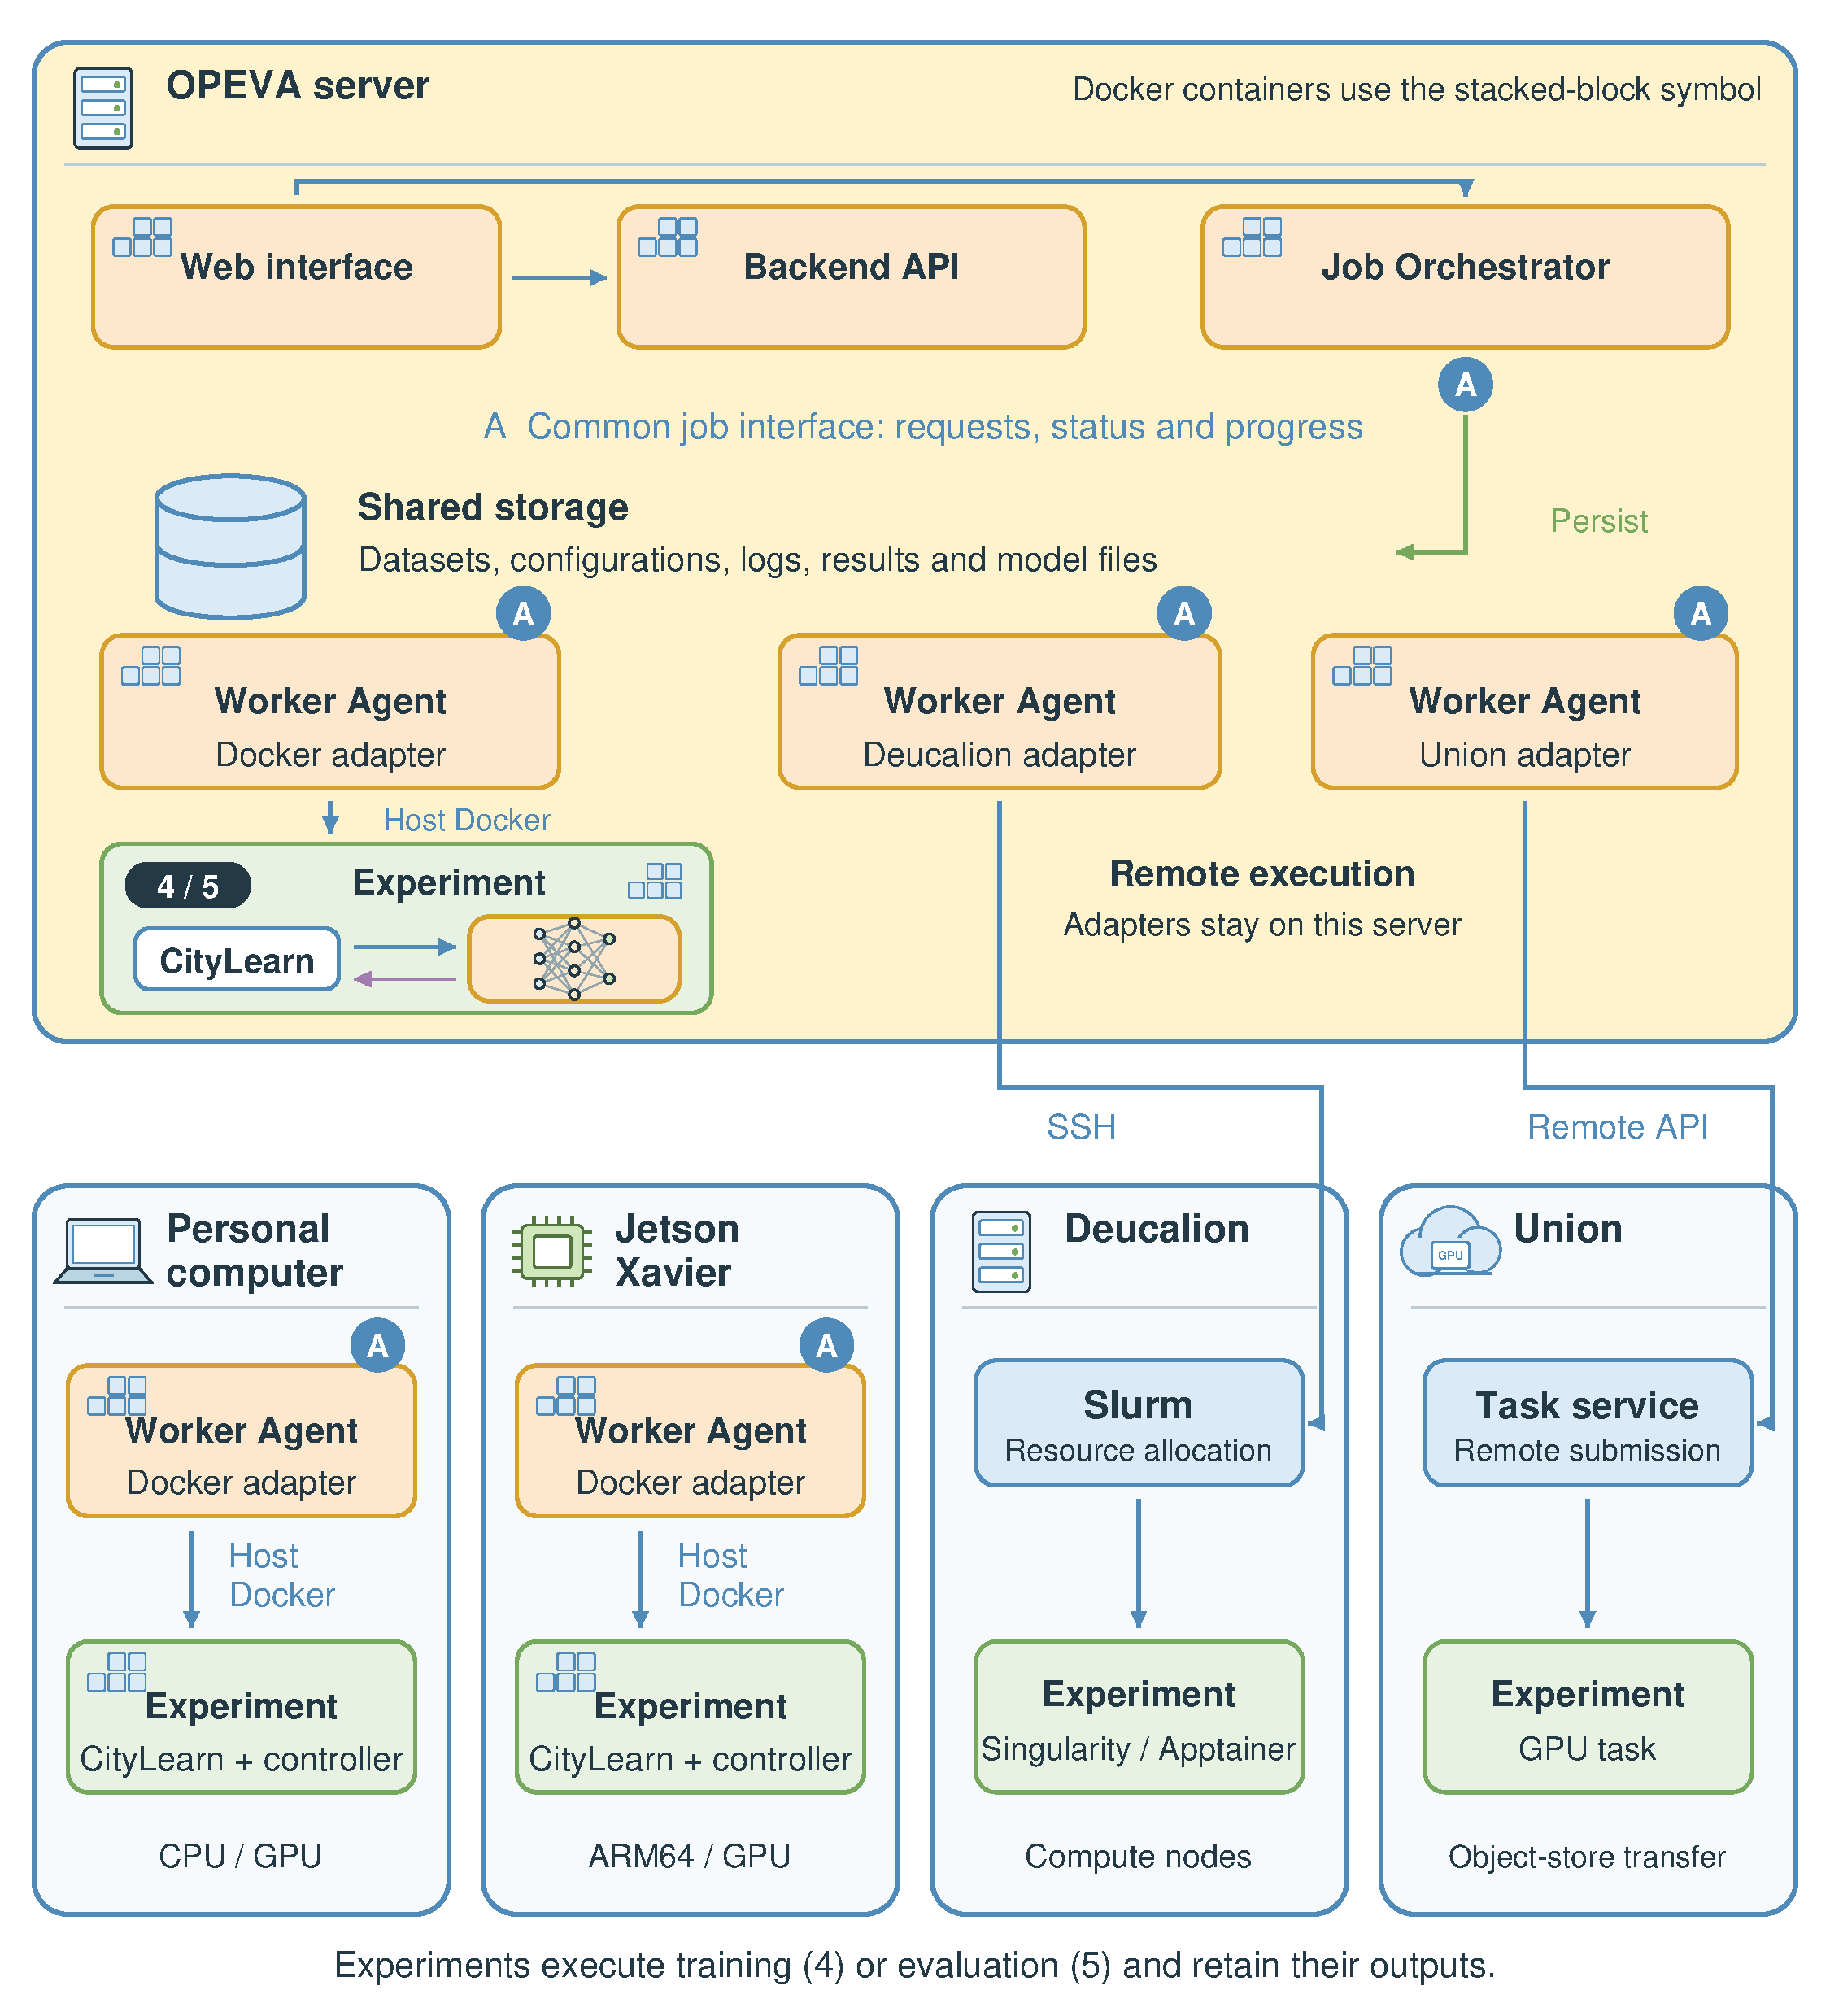
\includegraphics[width=\linewidth]{energaize-orchestration.pdf}
\caption[Computing infrastructure for experiment orchestration.]{Worker Agents manage training~(4) and evaluation~(5) on local or remote resources. The expanded experiment retains the simulator and controller of \cref{fig:energaize-development}.}
\label{fig:energaize-orchestration}
\end{figure}

The worker is a persistent service responsible for obtaining work, launching it, and reporting its progress. The experiment is the process that runs the simulator and control method for one job. With Docker execution, the worker and experiment occupy separate containers on the same host; access to the host's Docker service allows the worker to start and stop the experiment. A remote adapter performs the equivalent management through the target's submission interface. This division allows the experiment software to retain its own dependencies and execution environment while the worker manages its lifecycle.

The experiment configuration combines the \gls{rec} configuration and dataset with the selected controller, observations, actions, reward, random seed, and training or evaluation period. The execution request adds the software image and computing requirements. Resolving these settings before dispatch gives the worker a complete description of the work to perform. The configuration actually executed is retained with the job, so that a later change to a reusable configuration file does not change the account of an earlier experiment.

For the charging example, two runs may use the same controller and household data while assuming different departure times or charging limits. Their interpretation depends on keeping those differences visible. A retraining run likewise has its own configuration and record, even when it continues from an earlier model.

\begin{samepage}
Experiment tracking, model storage, and serving are established concerns in machine-learning operations \parencite{kreuzberger2023mlops,zaharia2018mlflow}. \gls{rl} also requires the environment in which experience is generated \parencite{li2022rlops}. The experiment record therefore retains the simulator and scenario configuration alongside the controller settings.

\end{samepage}

The orchestrator is implemented as a \gls{http} service using FastAPI. Its interface supports experiment submission, job inspection, worker communication, and access to configurations and results. Shared storage retains each job's settings, state, and outputs under a common identity used by the web interface and workers. The experiment can therefore continue independently of the browser session through which it was submitted.

A worker periodically reports its availability, software version, active work, and relevant computing capabilities. When it has capacity, it requests a job that matches its execution profile. The orchestrator supplies the software image, resolved configuration, execution command, and required data locations. The worker then launches the simulator and controller using the execution mechanism of its target. The algorithms receive the configuration prepared for the experiment, while the worker handles the surrounding execution process.

This separation gives each service a clear responsibility. Queueing and job identity remain with the orchestrator; resource-specific execution remains with the worker. The training program can consequently run on a local machine or through a remote scheduler using the same experiment description. Additional workers make it possible to execute independent experiments concurrently, including different random seeds, controller settings, or scenarios.

\subsection{Execution on Heterogeneous Computing Resources}
\label{sec:energaize-compute}

The computing resources used during development have different execution environments. A workstation can start a container directly, a supercomputer admits work through a batch scheduler, and a remote service may require data to be transferred before execution begins. The Worker Agent accommodates these differences through target-specific adapters. Each adapter carries the common job description into the target environment and returns its state and outputs to the orchestrator.

\Cref{tab:lifecycle-targets} summarises the supported execution profiles. The distinction between them concerns how the experiment reaches the processor, obtains its data, and returns its results. The scenario and controller settings remain attached to the same job throughout this process.

\begin{table}[htbp]
\centering
\caption{Computing resources and their execution adapters.}
\label{tab:lifecycle-targets}
\small
\renewcommand{\arraystretch}{1.12}
\begin{tabularx}{\textwidth}{@{}>{\raggedright\arraybackslash}p{0.20\textwidth}>{\raggedright\arraybackslash}p{0.25\textwidth}>{\raggedright\arraybackslash}X@{}}
\toprule
\textbf{Resource} & \textbf{Execution mechanism} & \textbf{Responsibility of the adapter} \\
\midrule
Server & Docker with shared storage & Start the selected image, provide data access, and collect outputs. \\
Personal computer & Docker with optional \gls{gpu} & Connect an intermittently available resource and complete active work before shutdown. \\
Deucalion & Slurm and Singularity/Apptainer & Stage inputs, submit the batch job, follow scheduler state, and retrieve results. \\
Union \gls{inesctec} & Remote tasks with \gls{gpu} resources & Transfer inputs, retain the remote run identity, and recover the returned results. \\
Jetson Xavier & Docker with a compatible NVIDIA image & Match the ARM64 architecture and installed \gls{gpu} software to the execution image. \\
\bottomrule
\end{tabularx}
\end{table}

For server and personal-computer workers, the experiment container reads the configuration and data from mounted storage. For Deucalion, the Worker Agent remains on the submission side. Its adapter creates a remote workspace, stages the required inputs, and submits a Slurm request using a compatible container image. Slurm allocates the computing resources on which the experiment runs through Singularity or Apptainer. Scheduler limits and resource requests become part of that execution setup. Logs are synchronised while the job runs, and the final outputs return to the job's stored record.

The Union Worker Agent similarly remains on the \gls{opeva} side and submits remote tasks. Inputs and results pass through object storage. The worker retains the remote run identity so that monitoring and result retrieval can continue across interruptions. The Jetson profile addresses another form of heterogeneity: its processor architecture and installed \gls{gpu} software require a compatible image. These differences are handled at the worker boundary, where the information needed to execute the experiment is available.

Keeping the adapters behind the common worker interface allows the computing infrastructure to grow without introducing a separate experiment format for each resource. It also preserves information about where and how a result was produced. The software image, execution target, and returned logs remain available when interpreting differences between runs or preparing a further experiment.

\subsection{Job Progress, Results, and Recovery}
\label{sec:energaize-job-recovery}

An experiment passes through several stages before its results are available. After submission and queueing, a worker accepts the job, prepares its execution environment, and starts the training or evaluation process. The job record follows this progression through explicit states. Remote preparation has its own place in that record because transferring a dataset or waiting for a scheduler is different from running the controller inside the simulator.

Progress updates and logs make this distinction useful to the operator. The EnergAIze web interface displays the queue, worker availability, execution state, training progress, and completed outputs. It also provides access to configurations and \gls{kpi} comparisons, with links to MLflow records where tracking is enabled. These views connect the visible result to the experiment that produced it. For a charging study, the operator can inspect cost and peak demand alongside the departure charge, then return to the corresponding scenario and controller settings.

Persistent state also supports recovery when communication or execution is interrupted. Each dispatched attempt can carry an identifying token that the worker returns with its updates. If a job is reassigned, updates from the superseded attempt are rejected. This prevents a delayed worker from replacing the state or results of a newer execution. A stop request follows the same division of responsibility: the orchestrator records the request, and the worker stops the container or remote job that it manages.

Remote result retrieval requires particular care. A training process may finish successfully while the connection needed to download its outputs is unavailable. In the Union adapter, a recovering state records this interval between completed computation and locally available results. The remote run identity and recovery progress are persisted, allowing the transfer to resume after the worker restarts. The completed training outputs can then be recovered without repeating the experiment. Deucalion similarly retains the connection between the local job and the remote scheduler record while its adapter monitors execution and retrieves the outputs.

Once execution and result retrieval are complete, model selection can use the recovered evidence. The selected controller then needs a description that allows the inference service to reconstruct the input processing and action interpretation used during evaluation. This is the role of the model contract.

\subsection{The Model Contract}
\label{sec:energaize-contract}

The selected model is exported with a model contract that preserves its input and output settings: observation names, ordering and encoding, returned actions, and agent--model associations. This manifest and the model files form the \emph{model bundle}~(6) shown in the development and deployment views. The full experiment configuration remains in the job record.

\Cref{tab:energaize-model-contract} groups the information passed through this interface. The installation configuration supplies the connection to physical equipment and its provider interfaces. The model contract supplies the interpretation required by the selected controller. Their correspondence is what allows an observation assembled by Percepta to reach the intended input and a returned action to be directed to the correct resource.

\begin{table}[htbp]
\centering
\caption{Information carried by the model contract.}
\label{tab:energaize-model-contract}
\small
\renewcommand{\arraystretch}{1.12}
\begin{tabularx}{\textwidth}{@{}>{\raggedright\arraybackslash}p{0.24\textwidth}>{\raggedright\arraybackslash}X>{\raggedright\arraybackslash}X@{}}
\toprule
\textbf{Part of the contract} & \textbf{Stored information} & \textbf{Use in runtime} \\
\midrule
Observations & Names, ordering, and input encoders & Reconstruct the input representation used during development. \\
Actions & Names, bounds, and output settings & Return identifiable actions in the form expected by the integration path. \\
Agents and models & Agent indices, model format, and file locations & Select the model associated with the requested agent. \\
Origin and configuration & Run identity and accompanying environment metadata & Associate the loaded controller with its development record. \\
\bottomrule
\end{tabularx}
\end{table}

For the household vehicle, the contract determines where \gls{soc} enters the model and how the returned charging decision is named. If the model was trained with encoded calendar variables or a particular observation order, the inference service reconstructs that processing when it loads the bundle. A controller serving several agents also needs the association between each agent and its model. This association can point to separate model files or to a shared model used by several agents.

The general export path produces neural models in the \gls{onnx} format and rule-based policies in \gls{json}. Before the bundle is finalised, validation checks the manifest structure, declared formats, referenced files, agent indices, and observation and action dimensions. The resulting package can be passed from the experiment implementation to the inference service without manually rebuilding its feature ordering or action mapping. The control methods developed in Chapters~\ref{chap:control-benchmark} and~\ref{chap:ti-marl} supply any additional requirements for their runtime components.

\subsection{Controller Deployment and Updates}
\label{sec:policy-registry}
\label{sec:edge-deploy}
\label{sec:lifecycle-monitoring}

The deployment backend maintains a catalogue of model bundles in shared storage. Each stored bundle retains its manifest and model files under a content-derived identity. The web interface allows the operator to inspect the available bundles and select a version for an inference target. A target is the service endpoint at which the selected controller will be loaded; the installation configuration determines which observations and equipment are associated with that service.

\Cref{fig:energaize-deployment} continues from the same model bundle~(6), through catalogue storage~(7), operator selection~(8), and backend loading~(9). The controller runs inside the inference service, using the runtime connections shown in \cref{fig:energaize-overview}.

\begin{figure}[htbp]
\centering
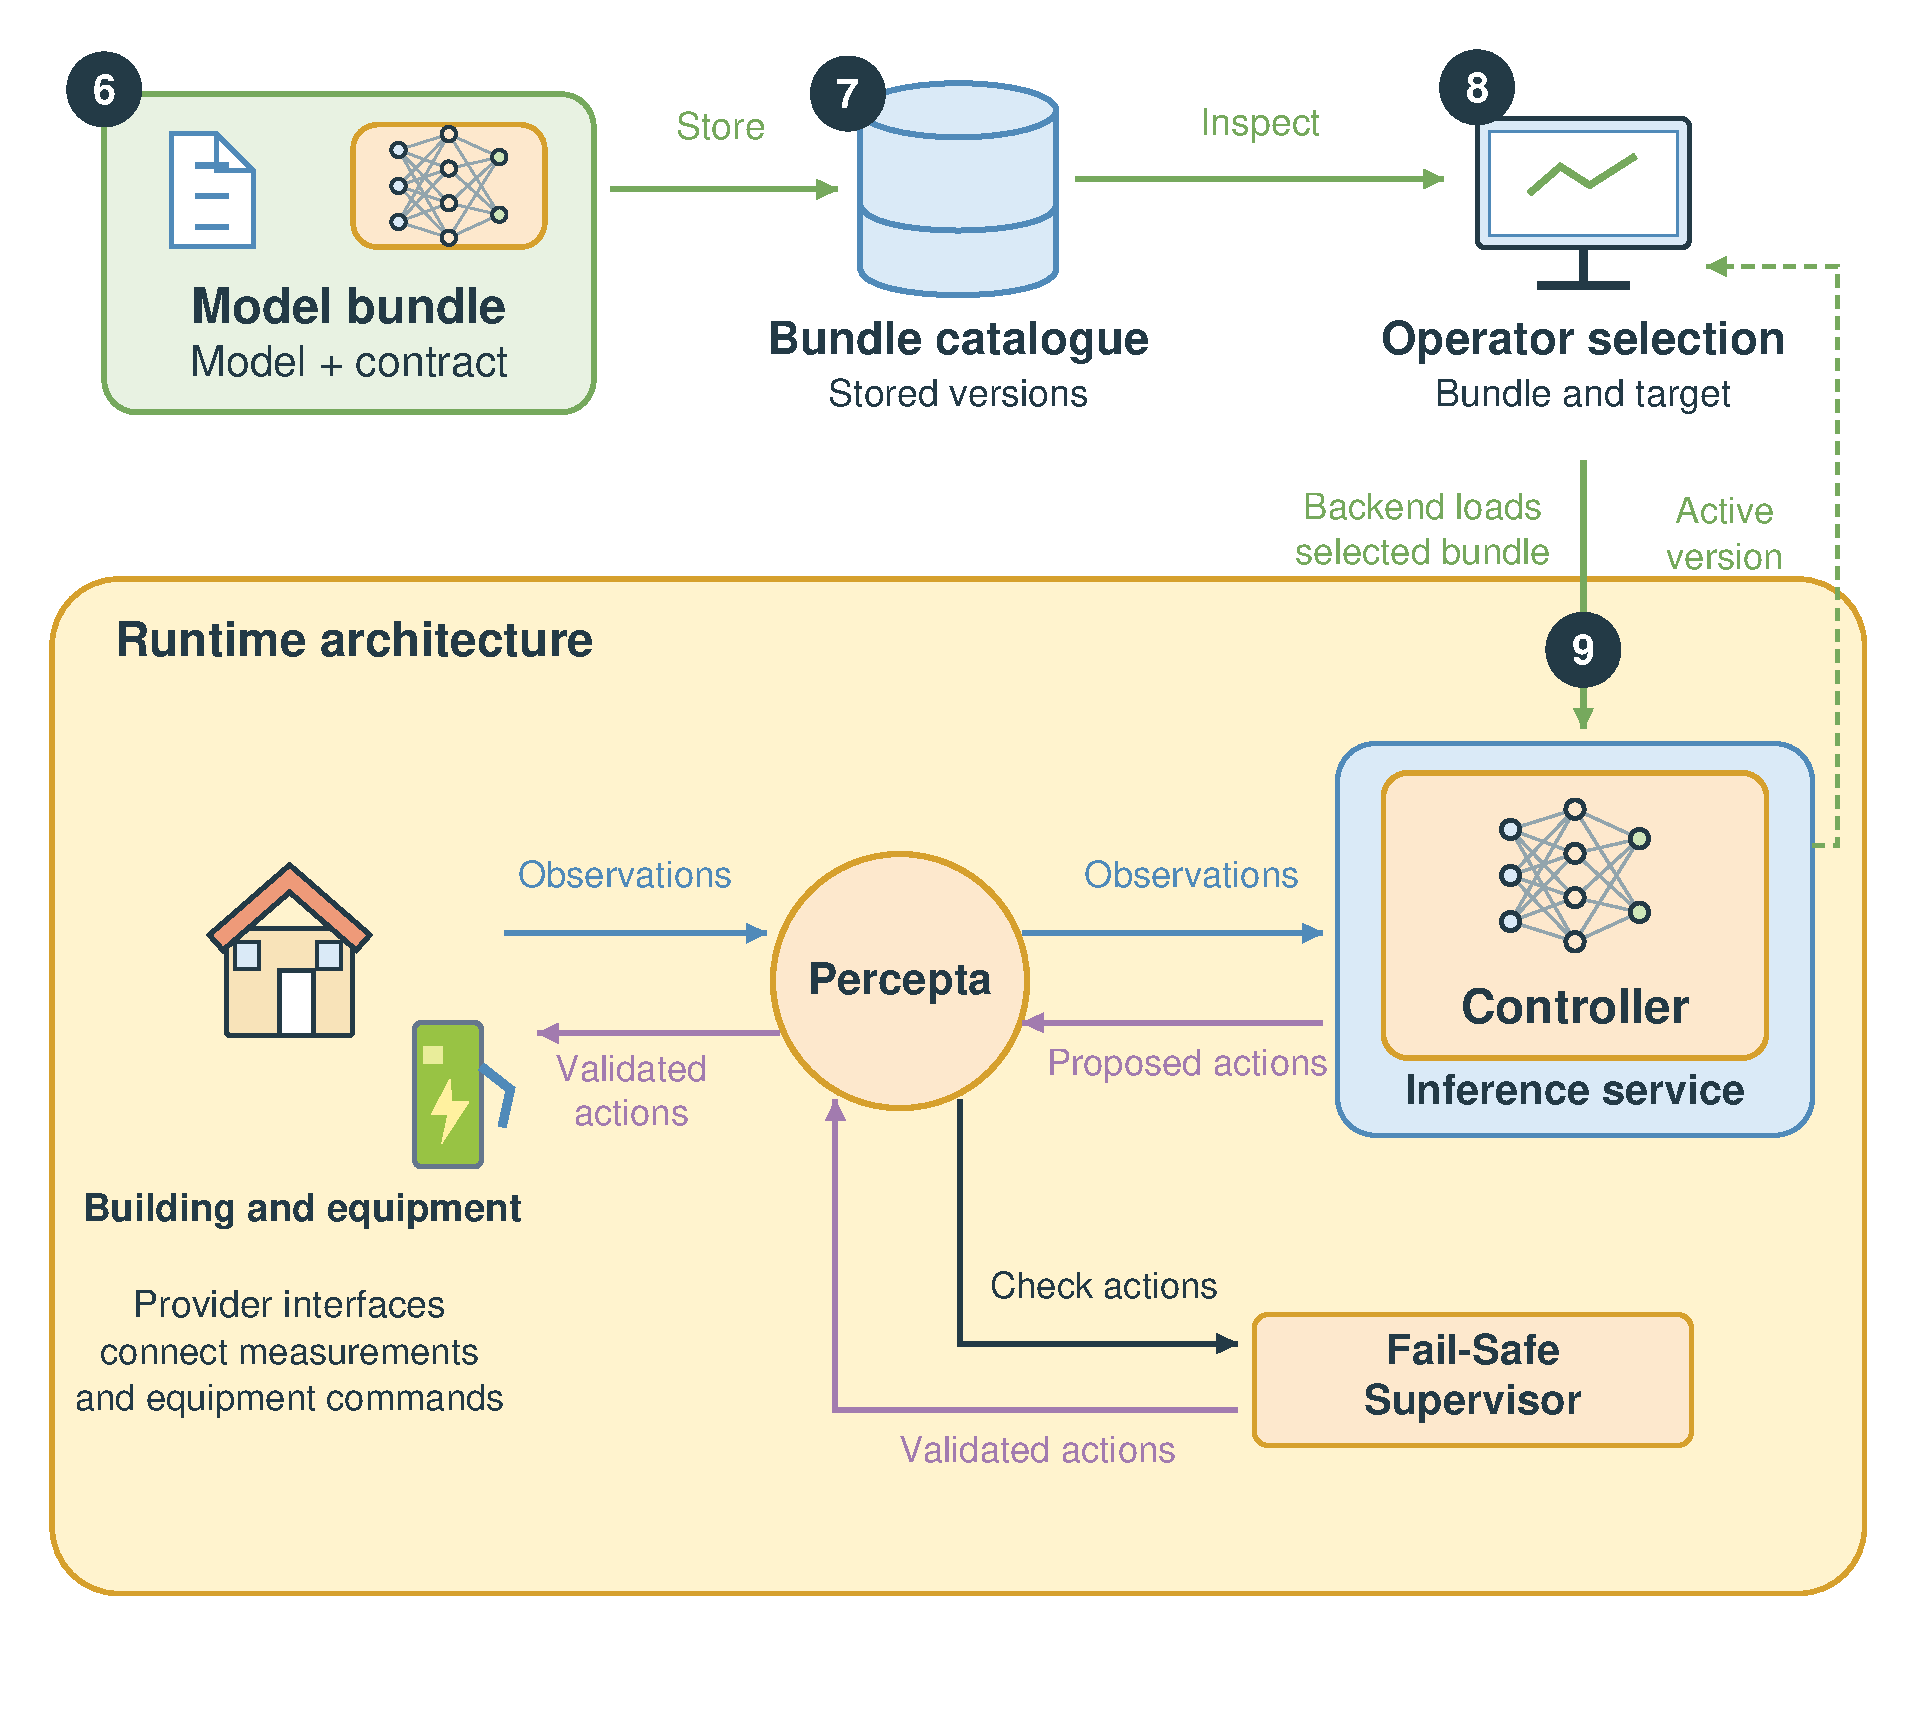
\includegraphics[width=\linewidth]{energaize-model-deployment.pdf}
\caption[Model deployment and the runtime control loop.]{Model deployment~(6--9) and the controller within the runtime control loop.}
\label{fig:energaize-deployment}
\end{figure}

For the selected target, the backend resolves the stored bundle location and sends a loading request to the inference service. The service reads the manifest, locates the model files, prepares the input encoders, and creates the appropriate \gls{onnx} or rule-based executor. It then reports the loaded configuration and agent indices, making the active controller visible to the backend and web interface.

During operation, health information exposes the service's readiness, while request identifiers associate inference calls with their responses. The records described in Section~\ref{sec:energaize-records} connect the loaded controller to supervisory interventions, provider responses, and subsequent measurements. An operator can consequently follow a charging request from the selected model to the power delivered at the installation.

Updates use the same loading path. The operator selects a new bundle for the target and inspects the reported active version after loading. Earlier bundles can remain in the catalogue and be selected again when a previous controller is required. The backend protects a bundle reported as active by a reachable target from deletion, preserving the files associated with that deployment. Each target exposes its own loaded state, allowing the operator to follow changes across installations.

The operational records retained during deployment supply the datasets and cases used for subsequent development. An operator can revisit intervals with repeated corrections or fallback use, together with changes in connection times, equipment, or operating limits. These findings guide scenario revisions, configuration updates, or controller retraining through the same orchestration service. The resulting candidate is evaluated through the process in Section~\ref{sec:energaize-training-evaluation}, after which the operator can select its model bundle for deployment. Its development record retains the connection to the operating conditions that motivated the update.

\section{Chapter Summary}
\label{sec:energAIze-forward-map}
\label{sec:energaize-chapter-map}

EnergAIze connects \gls{rec} energy control to the services needed to develop and operate its controllers. Runtime integrates observations, controller execution, independent supervision, and equipment interfaces. Development uses data and simulation to train and evaluate candidates, with the Job Orchestrator and Worker Agent managing experiment execution. The deployment backend loads the selected model bundle into the inference service. Operational records return measured outcomes and supervisory interventions to development, supporting later retraining and evaluation.

These connections give architectural form to the four dimensions established in Chapters~\ref{chap:introduction} and~\ref{chap:related-work}. For \emph{scalability}, \gls{rec} configurations and experiment records allow control outcomes to be related to the system's size, composition, and computing requirements. For \emph{deployability}, the model contract, development services, and equipment interfaces organise preparation, training and adaptation, integration, and maintenance so that evaluated behaviour can be reproduced and sustained. \emph{Safety} is addressed through constraint enforcement and separate records of proposals, supervisory intervention, and equipment response. \emph{Robustness} draws on service monitoring, fallback control, and recovery, with retained service examined under the conditions recorded during operation.

Chapter~\ref{chap:simulator} develops the simulation environment used to represent buildings and resources and compare their controllers. Chapters~\ref{chap:control-benchmark} and~\ref{chap:ti-marl} develop the control methods, while Chapter~\ref{chap:real-world} examines their integration and use in operating installations.

\setlength{\parskip}{\architectureoriginalparskip}
\clearpage
\setlength{\textfloatsep}{\architectureoriginaltextfloatsep}
\setlength{\intextsep}{\architectureoriginalintextsep}
\setlength{\abovecaptionskip}{\architectureoriginalcaptionskip}
\flushbottom
\clubpenalty=\architectureoriginalclubpenalty
\widowpenalty=\architectureoriginalwidowpenalty
